\documentclass[a4paper]{article}
\usepackage[noheadfoot,margin=2.5cm,a4paper]{geometry} 
\usepackage{amsmath, amsthm}
% \addtolength{\textheight}{20mm}
% \addtolength{\voffset}{-5mm}
\setlength{\footskip}{1cm}
\usepackage{graphicx}
\usepackage{url}
\usepackage{pgf}
%\usepackage{listings}
\usepackage{amsmath}

\graphicspath{{./images/}}


\title{Stereo Vision using the OpenCV library} \author{Sebastian
Dr\"oppelmann \\ Moos Hueting \\ Sander Latour \\ Martijn van der
Veen} \date{June 2010}
\begin{document}
%numbering for the equations and figures
\numberwithin{equation}{section}
\numberwithin{figure}{section}

\begin{titlepage}
  \maketitle
  \thispagestyle{empty}
\end{titlepage}

\tableofcontents 
\thispagestyle{empty}
\newpage

\section{Preface} 
Stereo vision is one of the key subjects in current computer vision
research. Stereo vision can be best described as taking two viewpoints
in a 3D world, comparing the distance between corresponding pixels
(representing objects) in both images and taking this distance as a
measurement for the real distance of the objects to the camera.
Such distance information is retrieved by a dense stereo
algorithm of which the output is often a disparity depth map. A
disparity depth map is a 2D image where the color of each pixel represents 
the distance of that point to the camera. In other words, light pixels are near
and dark pixels are far.

Depthmaps are interesting because they can be used for various
purposes:
\begin{description}
 \item[3D modeling of 2D images] When you take two 2D images of a 3D
environment and calculate the depthmap, you can create a 3D model of
the scene by using the depth as the third dimension.
 \item[Recognizing front objects] When you apply segmentation based on
the depthmap, you can distinguish objects that are situated in the
front of the scene.
 \item[Tracking of objects] When you have a depthmap it is easier to
track an object because you have additional segmentation
possibilities. You can create segments of pixels that are near based
on the depth of the pixels and their adjacency.
 \item[As information about the environment in path planning] A
depthmap supplies additional information for path planning.
\end{description}

\section{Theory}

\subsection{Camera calibration}
Cameras have some parameters that defines how real-world objects are
projected on the image plane. The four most important parameters define
the \emph{focal length} in $x$ and $y$ direction and the \emph{possible 
displacement} of the imagecenter away from the optic axis. The focal length
ideally is the distance between the \emph{center of projection} ($C1$ and
$C2$ in \ref{fig:rectepipole}) and the \emph{image plane} ($R1$ and $R2$).
These parameters are summarized in the following (homogeneous) matrix,
which is called the \emph{intern camera matrix}:
\[ \left( \begin{array}{ccc}
f_x & 0   & c_x \\
0   & f_y & c_y \\
0   & 0   & 1
\end{array} \right)\] 
If we choose a real-world coordinate system different from the coordinate
system centered at the cameras center of projection, we have another matrix,
called the \emph{extern camera matrix}, which defines the transformation from
this coordinate system to the camera coordinate system. This second matrix
contains rotations in the $x$, $y$ and $z$ direction, and a translation.
This alternative coordinate system becomes handy later on, when we will
choose our own coordinate system based on the chessboard.
Together, the intern and extern camera matrix form the basis for our
mathematical model of the camera, and could be used to calculate the 3D
real-world coordinates out of the 2D image coordinates, and vica versa.
Calibration tries to determine the parameters in these matrices.

When working with camera's and in particular cheap webcams, often there
will be some distortion of the grabbed images due to imperfections of
the camera. The two most important distortions are radial distortion,
caused by a lens being more spherical than the ideal parabolic lens would
be, and tangential distortion, caused by the lens not being fully parallel
to the image plane. Fortunately, both distortions can be resonable undone
with a simple mathematical reprojection. The distortions can be
characterized by a Taylor series of two terms for the lens shape and a
reprojection for the skew image plane. For brevety, we omit the mathematical
formulas and refer the interested reader to the OpenCV book
\cite{LearningOpenCV}.

The (five) parameters needed to undo the distortion can be calculated if we
could find a raster of points that lay on straight lines in the real world.
For this purpose often a chessboard pattern on a flat surface is used.
Based on the distorted raster found in one picture of a chessboard pattern
one could determine both distortions and, by using the determined parameters,
mathematically reconstruct all original images made with the camera.

When working with \emph{stereo} vision we also need to know the spatial
relation between the two cameras. Using the algorithm proposed by Zhang
\cite{zhang1999} we can automate this process by showing both cameras
different orientations of the same chessboard. A simple cornerfinding algorithm
can recognize the black-white intersections of the chessboard squares, see
also section \ref{chessboardcorners}.

The chessboard used can be of any size N by M. This way for each image
containing a chessboard we have $N*M$ points for which we know the image
coordinates in both cameras. Using the disparities of these points between
both cameras, we can estimate the rotation/translation matrix (called $E$)
which transforms the coordinate system of the left camera to the coordinate
system of the right camera, or the other way around. Using this transformation,
we could transform the physical coordinates of an object as seen by the left
camera to the physical coordinates as seen by the right camera.
The OpenCV stereo calibration function will also calculate a matrix (called
$F$) which could transform (2D) image pixel coordinates from left to right
image, or vica versa.

We have chosen not to describe the calibration algorithm fully here.
See the article by Zhang for more information \cite{zhang1999}.

\begin{figure}[h!bt]
  \centering
  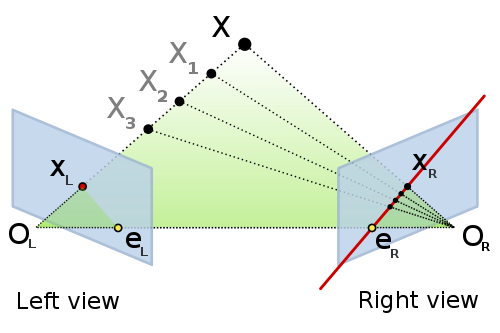
\includegraphics[width=0.4\textwidth]{epistandard}
  \caption{Epipolar geometry}
  \label{epi}
\end{figure}

\subsection{Epipolar geometry and rectification}
\label{recttheory}
\emph{Epipolar geometry} (figure \ref{epi}) is used in stereo vision to limit
the searching space when looking for matching points in both images. A point $X$
in 3D space is seen in the left view, which we will call the source image, as a
point $x$, which is on the line between the left camera's focal point $O_L$ and
point $X$.  This line is seen in the right view, which we will call the search
image, as a line. This is called an \emph{epipolar line}. Given both the cameras
internal and external matrices and a point $x_A$ we can generate an epipolar
line corresponding to this point in the search image. This constrains the search
space to this 1D line. However, this means that for each pixel in the source
image, we have to calculate the corresponding epipolar line in the search image.
It would be much more convenient if each epipolar line was on the same line as
the pixel it corresponded to. It is possible to transform the images in such a
way that the epipolar lines are parallel and horizontal, and that process is
called rectification.

Figure \ref{fig:rectepipole} demonstrates the process of rectification.  The
points $E_{1}$ and $E_{2}$ are called the \emph{epipolar points} of both
images. All epipolar lines intersect the epipolar point of a given image.
However, when the retinal planes of both cameras lie on the same plane, the
epipolar points move to infinity and the epipolar lines in one image become
parallel to one another. The line between the optical centers of both retinal
planes is called the baseline. When the epipolar points lie at infinity, we can
see that the epipolar lines are parallel to this baseline. That means that if
the baseline is parallel to the X-axis, the epipolar lines are horizontal.

\begin{figure}[h!]
\centering
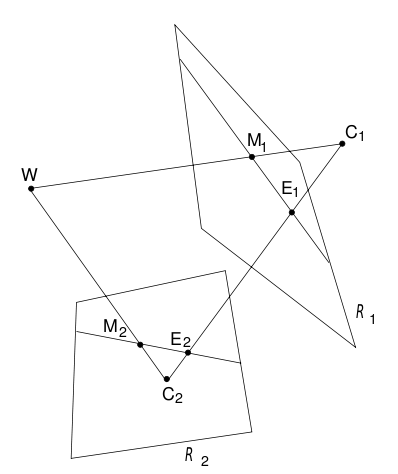
\includegraphics[width=0.4\textwidth]{nonrectepipole}
$\rightarrow$
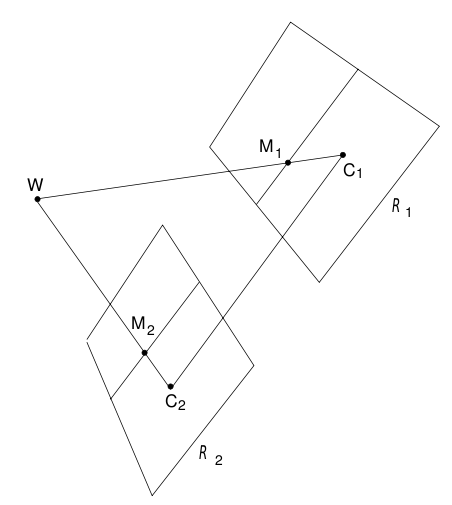
\includegraphics[width=0.4\textwidth]{rectepipole}
\caption{Left: unrectified cameras, right: rectified cameras. W represents the
point in 3D space, $C_1$ and $C_2$ represent the camera focal points, $M_1$ and
$M_2$ are the projections of $W$ on the retinal planes of the cameras and $R_1$
and $R_2$ are the retinal planes of the cameras. In the left image, the points
$E_1$ and $E_2$ represent the epipolar points of both images. In the right view,
these points lie at infinity. After rectification, the epipolar lines are colinear and horizontal}
\label{fig:rectepipole} \end{figure}

\subsubsection{Algorithm}
We will give the basic gist of the rectification algorithm here. 

\begin{enumerate}
  \item First both camera matrices are separately factorized into three parts:
  \begin{itemize}
    \item The internal camera matrix $A_o$
    \item The rotational matrix $R_o$ that gives the rotation between the camera's
    frame of reference and the world frame of reference
    \item The translation matrix $t_o$ that gives the translation between the
    camera's frame of reference and the world frame of reference
  \end{itemize}
  This means $P_o = A_o[R_o\ |\ t_o]$
  \item The new rotational matrix $R_n$ is constructed. This matrix makes
  sure that in the new `cameras' reference systems, the x-axis is parallel
  to the baseline. The baseline is simply the line between the two optical
  centers, which can be retrieved from $P_o$.
  \item The new internal camera matrix $A$ is constructed. This can be
  chosen arbitrarily and in this algorithm the mean between both original
  inner camera matrices ($A_{o1}, A{o2}$) is used.
  \item The new camera matrices are now $P_{n1} = A[R\ |\ -R c_1]$ and
  $P_{n2}
  = A[R\ |\ -R c_2]$. The optical centers are unchanged.
  \item A mapping is created that maps the original image planes of $P_{o1},
  P_{o2}$ to the new $P_{n1}, P_{n2}$. Because in general the pixels in the new
  images don't correspond to integer positions in the old images, bilinear
  interpolation is used to fill up the gaps.
\end{enumerate}

For a complete and in depth description of each step, please see
\cite{fusiello2000}.

\subsection{Dense Stereo} 
\label{theory}
Dense stereo combines the two images you get from the rectification process and
takes the position of the pixels in the left image to output the corresponding
pixel location in the right image. With this method we calculate the pixel's
distance from the camera.  The depth is then translated to a depth map where
points closer to the camera are almost white whereas points further away are
almost black. Points in between are shown in gray-scale, which get darker the
further away the point gets from the camera. See Figure \ref{dm_example} for an
example depth map with the original image. To achieve this, a whole list of
algorithms that do the trick is available.\footnote{A good overview can be found
at http://vision.middlebury.edu/stereo/eval/}

\begin{figure} \centering
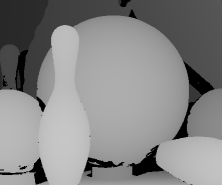
\includegraphics[width=0.3\textwidth]{depthmap}
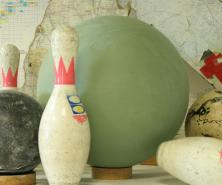
\includegraphics[width=0.3\textwidth]{depthmap_original}
\caption{A depthmap with the corresponding picture, gray values show
  the depth of the image}
\label{dm_example}
\end{figure}

Most of these algorithms are based on 4 principles:
\begin{itemize}
\item Graph Cut
\item Believe Propagation
\item Region Based / Block Matching
\item Dynamic Programming
\end{itemize}

The algorithms we are using are namely:
\begin{itemize}
\item Graph Cut
\item Block Matching
\item Semi Global Block Matching
\end{itemize}

These algorithms have to deal with the some problems in their
calculations. The main task of dense stereo algorithms is to find the
corresponding pixels in the match image starting from pixels in the
base image. While doing this the algorithms have to keep track of
occluded pixels, which are pixels that are found in one of the two images but
not in the other. 

\subsubsection{Matching}
\begin{figure} [h!tb]
\centering
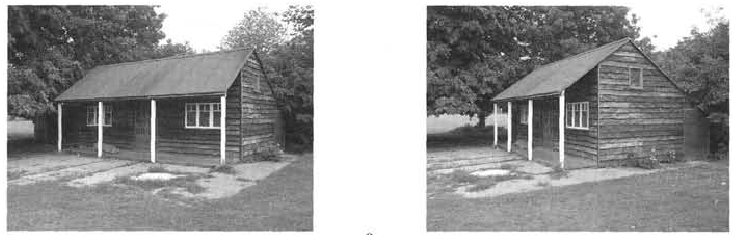
\includegraphics[width=0.8\textwidth]{matching_problems_direction}
\caption{On the left image the window is completely on the left of the
  rightmost pole, whereas in the right image, the window is completely
  on the right side of the rightmost pole}
\label{dirprob}
\end{figure}

% TODO SANDER: General disparity verhaal
The main goal of a dense stereo algorithm is matching one point in one
image to the corresponding point in the other image. During the
matching there are several tasks that the algorithm has to perform. At
first it has to compare the epipolar lines of the images pixel by
pixel. For every pixel on one line you have to find the counterpart on
the corresponding epipolar line in the other image. Often the pixels
aren't in the same order, for example if there is a lamp pole in front
of a house, things that lie on the left side of the lamp pole in the
left picture could sit on the right side in the right picture. See
figure \ref{dirprob}.

\begin{figure} [h!tb]
\centering
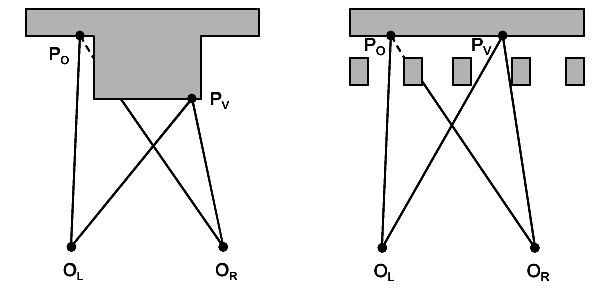
\includegraphics[width=0.6\textwidth]{matching_problems_occlusion}
\caption{Two examples of occlusion problems when working with stereo
vision}
\label{occprob} 
\end{figure}

Another problem is occlusion of pixels. As we can see in figure \ref{occprob},
in both examples pixel $P_O$ is visible for camera $O_L$, but is occluded in the
view of camera $O_R$. This has to be caught and handled. 

Because the OpenCV library that we have chosen has the basic
implementation of a \emph{Graph Cut} algorithm from
Kolmogorov\cite{kolmogorov2003}, we will start with that specific
algorithm. It is not the best algorithm for this task but because of
his general usability and it's high profile it is a good algorithm to start
with. Furthermore we will test the implementations of the
standard \emph{Block Matching} algorithm, which is faster but not that
precise. Also we will test a quite new implementation of the
\emph{Semi-Global Block Matching} algorithm, which was recently implemented in OpenCV.
% It is a bit slow and not the best algorithm to handle
% occlusion, but because it is easy to use we will at first use this
% algorithm and later replace it with an implementation of the block
% matching algorithms also provided by OpenCV.

\subsubsection{Graph Cut Theory}
\label{gc_theory}
Normal stereo matching algorithms try to match a pixel in the left image to a
pixel in the right image based on some individual property like color. Although
this is a fast and reasonably accurate process it does not deal with interlinear
consistency. An algorithm that incorporates interlinear consistency takes in
account the interpixel properties like adjacency. This results in a much more
accurate disparity depth map.  In order to maintain interlinear consistency you
want to connect horizontally adjacent pixels and add some sort of weight on that
connection to make it expensive to break. Furthermore you want to determine the
disparities in the entire picture that disrupt those neighbouring relations as
little as possible. \cite{zabih2001} states that given some energy function
you can construct a graph where the labeling with the lowest energy is equal to
the minimum cut on that graph. In that respect you can look at the stereo
correspondence problem as a labeling problem where you have to assign disparity
labels.  We will explain this in various sections below.\\\\

\begin{figure}[t] \centering
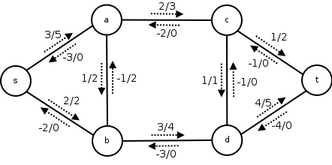
\includegraphics[width=180px]{Network_flow.png}
\caption{Flow network}
\label{flow_network}
\end{figure}
\noindent\textbf{Graph theory: Flow network basics}:\indent\\
Figure \ref{flow_network} shows a directed graph $\mathcal{G}$ which
can be formaly defined as $\mathcal{G} = \{\mathcal{V},\mathcal{E}\}$.
$\mathcal{V}$ depicts the set of vertices or nodes in the graph,
whereas $\mathcal{E}$ depicts the set
of edges between vertices. There are two special nodes S and T which are terminals.
Node S is a source terminal, which means that the incoming capacity is lower
than the outgoing capacity. Node T is a sink terminal, which has a higher incoming capacity than outgoing capacity.
The incoming and outgoing capacities of a node are distributed over the connected edges.
A \emph{graph cut} cuts edges in such a way that it disconnects the source from the sink, the cost of the cut equals the sum of the capacity of
the cut edges.\\\\
\noindent\textbf{Graph theory applied to stereo vision}:\indent\\
\begin{figure}[h!bt]
\begin{enumerate}
 \item Create a graph $\mathcal{G} = \{\mathcal{V},\mathcal{E}\}$
 \item $\forall_{p \epsilon \mathcal{P}}$ add $p$ to $\mathcal{V}$
 \item add terminals $f^0$ and $f^a$ to $\mathcal{G}$
 \item $\forall_{p,q \epsilon \mathcal{N}}$ add \{$p$,$q$\} to $\mathcal{E}$
 \item $\forall_{p \epsilon \mathcal{V}}$ add $\{f^0,p\}$ and $\{f^a,p\}$ to $\mathcal{E}$
 \item $\forall_{\{p,q\} \epsilon \mathcal{E}}$ set weight $w$ for $\{p,q\}$
\end{enumerate}
\caption{Steps for constructing a graph from picture $\mathcal{P}$}
\label{alg:gc_construct}
\end{figure}
Figure \ref{alg:gc_construct} describes the process of constructing a
graph $\mathcal{G}$ as discussed in the previous section from a
picture $\mathcal{P}$ of which the result is showed in figure \ref{fig:gc_end_result}.
The nodes represent pixels which can be reciprocally connected by edges.  $\mathcal{N}$ depicts a set of horizontally
adjacent pixel pairs.\\\\
\noindent\textbf{Weights}:\indent\\
\begin{equation}
 E(f) = E_{data}(f) + E_{smooth}(f) + E_{occlusion}(f)
\label{eq:energy}
\end{equation}
When two adjacent pixels have similar intensities it is likely that
they are part of the same object, this means that during the labeling
of disparities you would \emph{prefer} to assign the same label to
both pixels. This value corresponds to the $E_{data}$ term in equation \ref{eq:energy}.
$E_{smooth}$ measures the piecewise smoothness of the configuration and $E_{occlusion}$ 
adds a penalty for occluded pixels in the configuration.
The edge weights, such as $e(p,q)$ in figure \ref{fig:gc_end_result}, encode the energy function in such a way that it expresses
the likeliness that two pixels are part of the same object. In other words the higher the weight value 
the less you want to label the pixels with different disparities.\\
Every node is also connected to labeling terminals $f^a$ and $f^0$. These edges, such as $t^{\alpha}_{p}$, contain weights that 
express the costs of a pixel having that label. For more information on energy functions and weight values see \cite{zabih2001}.

\noindent\textbf{Cut}:\indent\\
The relation between the labeling configuration and the cut is described in equation \ref{eq: fC}. In plain english 
this means that a point $p$ is labeled $\alpha$ if the edge between $p$ and $\alpha$ is cut. The cost of that cut is equal 
to the sum of the weights of the cut edges. The idea of graph cut is to find the minimum cost cut. When a cut C cuts the 
edge between a point and a terminal and the edge between the adjacent connected point and the other terminal it also has to
cut the edge between the points, this will make the cost of the cut high if it cuts similar pixels.

\noindent\textbf{Iterations}:\indent\\
The implementation of graph cut in both \cite{zabih2001} and \cite{kolmogorov2003} is iterative. This means that each iteration 
pixels are labeled with one of two labels: the label they already had ($f^0$) or a new label ($f^{\alpha}$). The implementation 
will compare every disparity label in a given disparity range.\\\\

Suppose we have picture $\mathcal{P}$ as seen in \ref{fig:pictureP} with as ground truth (real disparity) configuration $f$.
Graph Cut will construct a graph as shown in figure \ref{fig:gc_end_result} and calculate the minimum cost cut in the graph.
As we can see in the result after the first iteration in figure \ref{fig:gcstep1} it has compared the new label $f^{\alpha} = 1$ with 
the initial label and determined that configuration $f$ in figure \label{fig:gcstep1} has the lowest costs. Figure \label{fig:gcstep2} shows 
the next iteration which shows a correct configuration.\\\\

%TODOSANDER
For a more in depth description of the graph cut algorithm, see
\cite{zabih2001}. For more details on the implementation in OpenCV,
see \ref{kolmogorov2003}.

\begin{figure}[h!bt]
\centering
\begin{minipage}[h]{.4\linewidth}
% Latex pgf picture
% Shows 5 pixels: {p,q,r,s,t}
% With bgcolors : {w,w,g,b,g}
\begin{pgfpicture}
\color{gray}
\pgfrect[fill]{\pgfxy(5,1)}{\pgfxy(1,1)}
\color{black}
\pgfrect[fill]{\pgfxy(4,1)}{\pgfxy(1,1)}
\color{gray}
\pgfrect[fill]{\pgfxy(3,1)}{\pgfxy(1,1)}
\color{black}

\pgfrect[stroke]{\pgfxy(5,1)}{\pgfxy(1,1)}
\pgfrect[stroke]{\pgfxy(4,1)}{\pgfxy(1,1)}
\pgfrect[stroke]{\pgfxy(3,1)}{\pgfxy(1,1)}
\pgfrect[stroke]{\pgfxy(2,1)}{\pgfxy(1,1)}
\pgfrect[stroke]{\pgfxy(1,1)}{\pgfxy(1,1)}

\pgfputat{\pgfxy(0.5,1.5)}{\pgfbox[center,center]{$\mathcal{P} =$}}

\pgfputat{\pgfxy(1.5,1.5)}{\pgfbox[center,center]{P}}
\pgfputat{\pgfxy(2.5,1.5)}{\pgfbox[center,center]{Q}}
\pgfputat{\pgfxy(3.5,1.5)}{\pgfbox[center,center]{R}}
\pgfputat{\pgfxy(4.5,1.5)}{\pgfbox[center,center]{\textcolor{white}{S}}}
\pgfputat{\pgfxy(5.5,1.5)}{\pgfbox[center,center]{T}}
\end{pgfpicture}
\end{minipage}
\hspace{.1\linewidth}
\begin{minipage}[h]{.4\linewidth}
% Latex pgf picture
% Shows 5 disparities: {2,2,1,0,1}
% With bgcolors : {w,w,g,b,g}
\begin{pgfpicture}
\pgfrect[stroke]{\pgfxy(5,1)}{\pgfxy(1,1)}
\pgfrect[stroke]{\pgfxy(4,1)}{\pgfxy(1,1)}
\pgfrect[stroke]{\pgfxy(3,1)}{\pgfxy(1,1)}
\pgfrect[stroke]{\pgfxy(2,1)}{\pgfxy(1,1)}
\pgfrect[stroke]{\pgfxy(1,1)}{\pgfxy(1,1)}

\pgfputat{\pgfxy(0.5,1.5)}{\pgfbox[center,center]{$f =$}}

\pgfputat{\pgfxy(1.5,1.5)}{\pgfbox[center,center]{2}}
\pgfputat{\pgfxy(2.5,1.5)}{\pgfbox[center,center]{2}}
\pgfputat{\pgfxy(3.5,1.5)}{\pgfbox[center,center]{1}}
\pgfputat{\pgfxy(4.5,1.5)}{\pgfbox[center,center]{0}}
\pgfputat{\pgfxy(5.5,1.5)}{\pgfbox[center,center]{1}}
\end{pgfpicture}
\end{minipage}
\caption{Picture $\mathcal{P}$}
\label{fig:pictureP}
\end{figure}
\begin{equation}
 f_{p}^{C} = \left\{
  \begin{array}{lll}
  \alpha & \text{if} & t^{\alpha}_{p} \epsilon \mathcal{C} \\ 
  f_{p}  & \text{if} & t^{\alpha}_{p} \epsilon \mathcal{C}
  \end{array}
\right.
 \forall p \epsilon \mathcal{P}
\label{eq: fC}
\end{equation}

\begin{figure}[h!bt]
\centering
% Latex pgf picture
% Shows graph of pixels {fa,p,q,r,s,t,f0}
% With label
\begin{pgfpicture}
\pgfsetlinewidth{1pt}
\pgfnodebox{p}[stroke]{\pgfxy(1,2)}{\textcolor{black}{P}}{4pt}{4pt}
\pgfnodebox{q}[stroke]{\pgfxy(3,2)}{\textcolor{black}{Q}}{4pt}{3pt}
\pgfnodebox{r}[stroke]{\pgfxy(5,2)}{\textcolor{black}{R}}{4pt}{4pt}
\pgfnodebox{s}[stroke]{\pgfxy(7,2)}{\textcolor{black}{S}}{5pt}{4pt}
\pgfnodebox{t}[stroke]{\pgfxy(9,2)}{\textcolor{black}{T}}{4pt}{4pt}

\pgfsetlinewidth{.5pt}
\pgfnodebox{f0}[stroke]{\pgfxy(5,0)}{$f^0$}{4pt}{4pt}
\pgfnodebox{a}[stroke]{\pgfxy(5,4)}{{$f^\alpha$}}{4pt}{4pt}

\pgfnodeconnline{p}{q}
\pgfnodeconnline{q}{r}
\pgfnodeconnline{r}{s}
\pgfnodeconnline{s}{t}

\pgfnodeconnline{f0}{p}
\pgfnodeconnline{f0}{q}
\pgfnodeconnline{f0}{r}
\pgfnodeconnline{f0}{s}
\pgfnodeconnline{f0}{t}

\pgfnodeconnline{a}{p}
\pgfnodeconnline{a}{q}
\pgfnodeconnline{a}{r}
\pgfnodeconnline{a}{s}
\pgfnodeconnline{a}{t}

\pgfnodelabel{a}{p}[0.4][-5pt]{\pgfbox[center,base]{$t^{\alpha}_{p}$}}
\pgfnodelabel{a}{q}[0.5][-5pt]{\pgfbox[center,base]{$t^{\alpha}_{q}$}}
\pgfnodelabel{a}{r}[0.6][-5pt]{\pgfbox[center,base]{$t^{\alpha}_{r}$}}
\pgfnodelabel{a}{s}[0.4][-8pt]{\pgfbox[center,base]{$t^{\alpha}_{s}$}}
\pgfnodelabel{a}{t}[0.3][-9pt]{\pgfbox[center,base]{$t^{\alpha}_{t}$}}

\pgfnodelabel{f0}{p}[0.4][-5pt]{\pgfbox[center,base]{$t^{0}_{p}$}}
\pgfnodelabel{f0}{q}[0.5][-5pt]{\pgfbox[center,base]{$t^{0}_{q}$}}
\pgfnodelabel{f0}{r}[0.6][-5pt]{\pgfbox[center,base]{$t^{0}_{r}$}}
\pgfnodelabel{f0}{s}[0.6][-8pt]{\pgfbox[center,base]{$t^{0}_{s}$}}
\pgfnodelabel{f0}{t}[0.5][-9pt]{\pgfbox[center,base]{$t^{0}_{t}$}}

\small
\pgfnodelabel{p}{q}[0.6][4pt]{\pgfbox[center,base]{$e(p,q)$}}
\pgfnodelabel{q}{r}[0.5][4pt]{\pgfbox[center,base]{$e(q,r)$}}
\pgfnodelabel{r}{s}[0.5][4pt]{\pgfbox[center,base]{$e(r,s)$}}
\pgfnodelabel{s}{t}[0.4][4pt]{\pgfbox[center,base]{$e(s,t)$}}

\end{pgfpicture}
\caption{Graph of a 5-pixel image with weights and labels $f^a$ and $f^0$}
\label{fig:gc_end_result}
\end{figure}

\begin{figure}[h!bt]
\centering
% Latex pgf picture
% Shows graph of pixels {fa,p,q,r,s,t,f0}
% With cut C, where:
% C = {p-fa,q-fa,r-fa,r-s,s-f0,s-t,t-fa}
\begin{pgfpicture}
\pgfsetlinewidth{1pt}
\pgfnodebox{p}[stroke]{\pgfxy(1,2)}{\textcolor{black}{P}}{4pt}{4pt}
\pgfnodebox{q}[stroke]{\pgfxy(3,2)}{\textcolor{black}{Q}}{4pt}{3pt}
\pgfnodebox{r}[stroke]{\pgfxy(5,2)}{\textcolor{black}{R}}{4pt}{4pt}
\pgfnodebox{s}[stroke]{\pgfxy(7,2)}{\textcolor{black}{S}}{5pt}{4pt}
\pgfnodebox{t}[stroke]{\pgfxy(9,2)}{\textcolor{black}{T}}{4pt}{4pt}

\pgfsetlinewidth{.5pt}
\color{black}
\pgfnodebox{f0}[stroke]{\pgfxy(5,0)}{$f^0$}{4pt}{4pt}
\pgfnodebox{a}[stroke]{\pgfxy(5,4)}{{$f^\alpha$}}{4pt}{4pt}

\pgfnodeconnline{p}{q}
\pgfnodeconnline{q}{r}
\color{red}
\pgfnodeconnline{r}{s}
\pgfnodeconnline{s}{t}
\color{black}

\pgfnodeconnline{f0}{p}
\pgfnodeconnline{f0}{q}
\pgfnodeconnline{f0}{r}
\color{red}
\pgfnodeconnline{f0}{s}
\color{black}
\pgfnodeconnline{f0}{t}

\color{red}
\pgfnodeconnline{a}{p}
\pgfnodeconnline{a}{q}
\pgfnodeconnline{a}{r}
\color{black}
\pgfnodeconnline{a}{s}
\color{red}
\pgfnodeconnline{a}{t}

\pgfsetdash{{0.2cm}{0.2cm}{0.2cm}{0.2cm}}{0cm}
\pgfsetlinewidth{1pt}

\pgfmoveto{\pgfxy(1,3)}
\pgflineto{\pgfxy(5.1,3)}

\pgfcurveto{\pgfxy(5.8,3)}{\pgfxy(5.9,2)}{\pgfxy(5.9,2)}
\pgfcurveto{\pgfxy(5.9,1.3)}{\pgfxy(6.5,1.3)}{\pgfxy(7,1.3)}
\pgfcurveto{\pgfxy(8,1.3)}{\pgfxy(7.8,2)}{\pgfxy(8.1,3.3)}

\pgfstroke
\pgfputat{\pgfxy(1.5,3.2)}{\pgfbox[center,center]{$\mathcal{C}$}}
\end{pgfpicture}
% Latex pgf picture
% Shows 5 disparities: {1,1,1,0,1}
% With bgcolors : {w,w,g,b,g}
\begin{pgfpicture}
\pgfrect[stroke]{\pgfxy(5,1)}{\pgfxy(1,1)}
\pgfrect[stroke]{\pgfxy(4,1)}{\pgfxy(1,1)}
\pgfrect[stroke]{\pgfxy(3,1)}{\pgfxy(1,1)}
\pgfrect[stroke]{\pgfxy(2,1)}{\pgfxy(1,1)}
\pgfrect[stroke]{\pgfxy(1,1)}{\pgfxy(1,1)}

\pgfputat{\pgfxy(0.5,1.5)}{\pgfbox[center,center]{$f =$}}

\pgfputat{\pgfxy(1.5,1.5)}{\pgfbox[center,center]{1}}
\pgfputat{\pgfxy(2.5,1.5)}{\pgfbox[center,center]{1}}
\pgfputat{\pgfxy(3.5,1.5)}{\pgfbox[center,center]{1}}
\pgfputat{\pgfxy(4.5,1.5)}{\pgfbox[center,center]{0}}
\pgfputat{\pgfxy(5.5,1.5)}{\pgfbox[center,center]{1}}
\end{pgfpicture}
\caption{Graph-Cut step 1 with $f^\alpha = 1$}                                             
\label{fig:gcstep1}
\end{figure}
\begin{figure}[h!bt]
\centering
% Latex pgf picture
% Shows graph of pixels {fa,p,q,r,s,t,f0}
% With cut C, where:
% C = {p-fa,q-fa,r-fa,r-s,s-f0,s-t,t-fa}
\begin{pgfpicture}
\pgfsetlinewidth{1pt}
\pgfnodebox{p}[stroke]{\pgfxy(1,2)}{\textcolor{black}{P}}{4pt}{4pt}
\pgfnodebox{q}[stroke]{\pgfxy(3,2)}{\textcolor{black}{Q}}{4pt}{3pt}
\pgfnodebox{r}[stroke]{\pgfxy(5,2)}{\textcolor{black}{R}}{4pt}{4pt}
\pgfnodebox{s}[stroke]{\pgfxy(7,2)}{\textcolor{black}{S}}{5pt}{4pt}
\pgfnodebox{t}[stroke]{\pgfxy(9,2)}{\textcolor{black}{T}}{4pt}{4pt}

\pgfsetlinewidth{.5pt}
\color{black}
\pgfnodebox{f0}[stroke]{\pgfxy(5,0)}{$f^0$}{4pt}{4pt}
\pgfnodebox{a}[stroke]{\pgfxy(5,4)}{{$f^\alpha$}}{4pt}{4pt}

\pgfnodeconnline{p}{q}
\color{red}
\pgfnodeconnline{q}{r}
\color{black}
\pgfnodeconnline{r}{s}
\pgfnodeconnline{s}{t}


\pgfnodeconnline{f0}{p}
\pgfnodeconnline{f0}{q}
\color{red}
\pgfnodeconnline{f0}{r}
\pgfnodeconnline{f0}{s}
\pgfnodeconnline{f0}{t}

\color{red}
\pgfnodeconnline{a}{p}
\pgfnodeconnline{a}{q}
\color{black}
\pgfnodeconnline{a}{r}
\pgfnodeconnline{a}{s}
\pgfnodeconnline{a}{t}

\color{red}
\pgfsetdash{{0.2cm}{0.2cm}{0.2cm}{0.2cm}}{0cm}
\pgfsetlinewidth{1pt}

\pgfmoveto{\pgfxy(1,3)}
\pgflineto{\pgfxy(3.1,3)}

\pgfcurveto{\pgfxy(4.3,3)}{\pgfxy(4.4,2)}{\pgfxy(4.4,2)}
\pgfcurveto{\pgfxy(4.4,1.3)}{\pgfxy(5,1.3)}{\pgfxy(5.5,1.3)}
\pgflineto{\pgfxy(10,1.3)}

\pgfstroke
\pgfputat{\pgfxy(1.5,3.2)}{\pgfbox[center,center]{$\mathcal{C}$}}
\end{pgfpicture}
% Latex pgf picture
% Shows 5 disparities: {2,2,1,0,1}
% With bgcolors : {w,w,g,b,g}
\begin{pgfpicture}
\pgfrect[stroke]{\pgfxy(5,1)}{\pgfxy(1,1)}
\pgfrect[stroke]{\pgfxy(4,1)}{\pgfxy(1,1)}
\pgfrect[stroke]{\pgfxy(3,1)}{\pgfxy(1,1)}
\pgfrect[stroke]{\pgfxy(2,1)}{\pgfxy(1,1)}
\pgfrect[stroke]{\pgfxy(1,1)}{\pgfxy(1,1)}

\pgfputat{\pgfxy(0.5,1.5)}{\pgfbox[center,center]{$f =$}}

\pgfputat{\pgfxy(1.5,1.5)}{\pgfbox[center,center]{2}}
\pgfputat{\pgfxy(2.5,1.5)}{\pgfbox[center,center]{2}}
\pgfputat{\pgfxy(3.5,1.5)}{\pgfbox[center,center]{1}}
\pgfputat{\pgfxy(4.5,1.5)}{\pgfbox[center,center]{0}}
\pgfputat{\pgfxy(5.5,1.5)}{\pgfbox[center,center]{1}}
\end{pgfpicture}
\caption{Graph-Cut step 2 with $f^\alpha = 2$}
\label{fig:gcstep2}
\end{figure}

\subsubsection{Semi Global Block Matching Theory}
Semi global block matching is built on the idea that you use mean data
from blocks of pixels as pixel energy and then build up a cost array
over the costs of all disparities from the minimum disparity to the
maximum disparity for all the pixels. Afterwards a search is done for
the minimum path cost in several directions of the image. The minimum
path cost is calculated from the pixel energy with penalties for the
disparity difference to neighbour pixels along a path that ends in the
pixel the disparity is searched for, where the one path with the
lowest cost is the right one. This is done on
subpixel level. After calculation of the disparities there are some
refinement steps to filter out peaks and noise.\\
The Middlebury page divides disparity algorithms mainly into four
parts, where some of the parts are optional. These parts are:
\begin{itemize}
\item cost computation
\item cost aggregation
\item disparity computation/optimization
\item disparity refinement
\end{itemize}
\noindent For the SGBM algorithm these steps are filled in as follows:\\
\textbf{Cost computation} can be done from the intensity or color
pixel values. Radiometric differences also have to be kept in mind, so
the gradient can also be calculated.\\
\textbf{Cost aggregation} connects the costs of the neighbourhood of
pixels to find the cheapest (thus matching) pixel in the compare
image. This is done through a global energy function from all
directions through the image.\\
\textbf{Disparity computation} calulates the real disparity from the
previously calculated energy through a winner-takes-all
implementation.\\
\textbf{Disparity refinements} are used to further stabilize the
disparity map. This is done via peak filtering, intensity consistent
disparity selection and gap interpolation. Also multibaseline matching
is done through the fusion of disparities to circumvent streaking and
add consistency. Because refinement is a separate part and has nothing
to do with stereovision per se, we leave it out in the explanation.\\

\emph{\textbf{Cost Calculation}}:\\
% the costs of this algorithm is caluclated from the intensity of the
% base pixel $I_{m\mathbf{p}}$ and the match pixel intensity
% $I_{m\mathbf{q}}$. Here the formula $\mathbf{q} = e_{bm}(\mathbf{p},
% d) = [p_x - d, p_y]^T$ is used where $d$ represents the disparity in
% rectified images. The size of the matching area can influence
% robustness of the images. Larger areas are more robust but fine
% structures are blurred more, because of the assumption of the same
% disparity over the whole area which isn't always true.
The \emph{matching cost} for the blocks of pixels used for calculating
the disparity in the OpenCV implementation are calculated through the
implementation of the subpixel algorithm described in the paper of
Birchfeld and Tomasi: "Depth Discontinuities by Pixel-to-Pixel Stereo"
\cite{birchtom99}. This is done by finding the correspondence
$I_{m\mathbf{q}}$ of the matching image from the mean intensity of a
block of pixels $I_{b\mathbf{p}}$ in the base image with the formula
$\mathbf{q} = \mathcal{e}_{bm}(\mathbf{p}, d)$ where
$\mathcal{e}_{bm}(\mathbf{p}, d)$ represents the epipolar line for
$\mathbf{p}$ in $I_b$. The size of the area has influence on the
robustness of the disparity map. Larger areas are more robust but fine
structures get more blurred, because of the assumption of the same
disparity over the whole area which isn't always true. The disparity
cost $C_{BT}( \mathbf{p},d)$ is calculated for a chosen squareblock of
pixels $\mathbf{p}$ from $minX$ till $maxX$ (the limits of the block),
where $d$ represents the current disparity in the rectified images and
$x$ is the pixel in the current block. \eqref{eq:costcalc} This is
done over all disparities between the given minimum and maximum
disparity $minD$ and $maxD$.\\
\begin{equation}
  \label{eq:costcalc}
  C_{BT}[(x-minX)*maxD - minD + (d - minD)]
\end{equation}
% For each pixel $row1[x], max(-maxD, 0) \leq minX \leq x < maxX \leq
% width - max(0, -minD)$, and for each disparity $minD \leq d < maxD$
% the function computes the cost $(C[(x-minX)*(maxD - minD) + (d -
% minD)])$, depending on the difference between $row1[x]$ and
% $row2[x-d]$.\\

\emph{\textbf{Cost Aggregation}}:\\ 
To smoothen wrong disparities calculated by the cost function and
finding the right ones, the Energy of the disparity image is
calculated from the sum of all pixel matching costs for the disparity
of $D$. Different penalties, $P_1, P_2$ are applied for small and
large disparity changes \eqref{eq:enerform}.
\begin{equation}
E(D) = \displaystyle\sum\limits_{\mathbf{p}}
(C_{BT}(\mathbf{p},D_\mathbf{p}) +
\displaystyle\sum\limits_{\mathbf{q} \in N_\mathbf{p}} P_1
T[|D_\mathbf{p} - D_\mathbf{q}| = 1] +
\displaystyle\sum\limits_{\mathbf{q} \in N_\mathbf{p}} P_2
T[|D_\mathbf{p} - D_\mathbf{q}| > 1]) 
%  \caption{Energy Formula}
  \label{eq:enerform}
\end{equation}
The 
penalty for small changes in disparity $P_1$ is a constant
whereas the penality for higher disparity changes $P_2$ is also used
to catch discontinuities on intensity changes. This can be done
through the use of the intensity of neighbouring pixels $\mathbf{p}$
and $\mathbf{q}$ in the base image $I_b$\eqref{eq:penalty}.
But it always has to be ensured that $P_1 \leq P_2$. Now matching
is '\textit{only}' a question of minimizing the Energy $E(D)$.
\begin{equation}
  \displaystyle\frac{P_{2}^{'}}{|I_{b\mathbf{p}}-I_{b\mathbf{q}}|}
\label{eq:penalty}
\end{equation}
%\emph{\textbf{Energy minimization}}:\\ 
Because 2D energy minimization would be a NP-complete problem, 1D
Computation is used which can be calculated in polynomial time. To
cover the equally important information of different directions of the
image, 1D lines from '\textit{all}' directions which end in the
pixelblock you are searching the disparity for, are considered (see
Figure \ref{fig:directions})
\begin{figure}
  \centering
  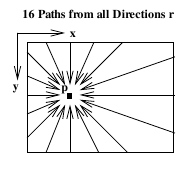
\includegraphics[width=0.3\textwidth]{directions}
  \caption{Directions of paths considered}
  \label{fig:directions}
\end{figure}
\noindent In the Hirschm\"{u}ller paper 8-16 paths
from all directions are recommended, whereas the standard algorithm in
OpenCV calculates 5 or 8 directions due to the high memory cost. For
our implementation we used 8 directions. For every path chosen the
smoothed path cost $S(\mathbf{p},d)$ is calculated through the
traversing path cost $L_{r}(\mathbf{p},d)$, were the cost represents
the energy formula \eqref{eq:enerform} along \textbf{an} arbitrary 1D
path \eqref{eq:trav}. Because the numbers can add up this way to
really huge numbers, the minimum path cost of the previous pixel $\mathit{k}$ is
substracted. This way the numbers stay smaller and the path doesn't
change it's minimum cost way, because the minimum cost of the pixel
before is a constant.  For precalculation all costs can be saved in an
integer array of size $[W*H*D]$ and the aggregated costs are then
saved in an equally sized array $S$.
\begin{align}
  \label{eq:trav}
  L_{r}(\mathbf{p},d) = 
  C_{BT}(\mathbf{p},d) + min(L_{r}(\mathbf{p} -
  \mathbf{r}, d), 
  \notag\\
  L_{r}(\mathbf{p} - \mathbf{r}, d - 1) + P_1,
  \notag\\
  L_{r}(\mathbf{p} - \mathbf{r}, d + 1) + P_1,
  \\
  \displaystyle\min\limits_{\mathit{i}} L_{r}(\mathbf{p} - \mathbf{r}, \mathit{i}) +
  P_2) -
  \displaystyle\min\limits_{\mathit{k}} L_{r}(\mathbf{p} -
  \mathbf{r}, \mathit{k})\notag
\end{align}

\emph{\textbf{Disparity Computation}}:\\
The base disparity map $D_b$ from the base image $I_b$ is caluclated by
picking the disparity with the minimum path cost for each pixel. This
is done with subpixel accuracy by picking the minimum of a quadratic
curve through the neighbouring pixel costs. The disparity map $D_m$ of
the match image from $I_m$ is calculated by traversing the epipolar
line of pixel $q$ in the match image. The disparity is then again the
disparity of the lowest pathcost. To enhance the quality of the
disparity map, you can calculate the disparities again but with $I_m$
as base image and $I_b$ as match image. After $D_m$ and $D_b$ have
been calculated, a consitency check is done between the two. If the
consistency between the two is too great (e.g. due to occlusion) the
disparity is set to invalid. Also unique constrained can be switched
on, which enforces one on one pixel mappings.

\section{Implementation}

\subsection{OpenCV}
\label{opencv} OpenCV is a library of programming functions for real
time computer vision. By using this library we can constrain our tasks
mostly to integrating various parts of OpenCV and expanding it where
necessary. If we would not use OpenCV, we would had to implement a lot
of basic computer vision functions, so there would probably be not
enough time to achieve our goal. OpenCV is fast library written in C/C++,
and has python binding as well, which we will use to decrease the risk
of programming errors.

\subsection{Calibration}
\label{calib_implement} OpenCV has a separate function for calibrating
a set of stereo cameras. This function\footnote{See stereoCalibrate in
the OpenCV documentation} uses as input a list of coordinates of
points in the left image and the coordinates of the same points in the
world in the right image, and a set of coordinates where these points
actually lie in the real world (3D coordinates).

\subsubsection{Chessboard points}
\label{chessboardpoints} As input for the calibration, we use
the intersection points of a chessboard. These points on the
chessboard are recognized by the stereo cameras and a list of
chessboard piececorners coordinates is returned, see Figure
\ref{chessboardcorners}. The corners are being found by by first
thresholding the image and then trying to locate a grid of black-white
transitions of the given count. This gives an approximation on pixel level,
which is not very accurate.

Because we are looking for the relationship between the two cameras and
not the relationship between a camera and the actual world, we can
choose the origin for these ``real world points'' however we like. As
we are using the chessboard, it is very convenient to choose the x and
y axes along the sides of the chessboard, so that the first
intersection lies at $(0, 0, 0)$ in the real world.

To improve the corner locations, one could use the FindCornerSubPix()
function, which uses Harris cornerdetection. To fully cover the
algorithm for this correction algoritm would require a lot of linear
algebra and isn't covered at that depth here\footnote{See the OpenCV
documentation, chapter 10, for the function findChessboardCorners for
mathematical background}. If the reader has no background in linear
algebra, the next paragraph can safely be skipped.

We give a short overview:
For each approximated location, which are pixel coordinates, make vectors
from some not yet determined subpixel location $q$ to other points $p$,
some pixels away from $q$. Take the dot-product of this vector with
the gradient vector for location $p$. This dot-product is equal
to zero in two situations: if $p$ is somewhere on a square, the gradient
vector and thus the dot-product is zero, and when $qp$ is located exactly
on an edge, the gradient vector is perpendicular to $qp$ and thus the
dot-product is zero. If $q$ is the correct subpixel corner location, then
all dot-products are zero. FindCornerSubPix() sets these dot-products to
zero and tries to solve the equations, the best solution for $q$ is the
new subpixel location.

%% NOTE: ik weet niet of dit wordt gebruikt, maar het klinkt als een goed
%%       algoritme voor corners vinden..
%\begin{enumerate}
% \item Make a second-derivative image, thus calculate the difference
%       of the difference in intensity for each pixel. High values
%       indicate edges.
% \item Calculate the so-called \emph{Autocorrelation matrix} and its
%       eigenvalues for a small window for each pixel.
% \item for which the Autocorrelation matrix has two large
%       eigenvalues are likely to be corners, which means these pixels
%       have an intersection of two edges
%\end{enumerate}


\begin{figure} [h!tb]
\centering
  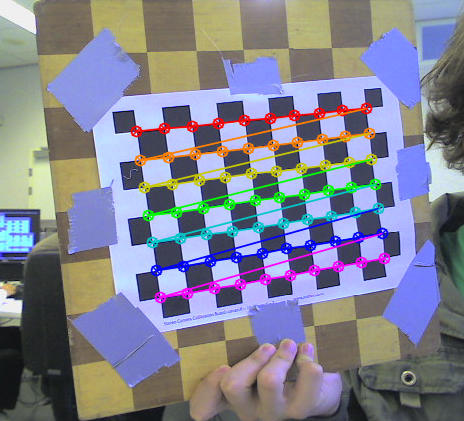
\includegraphics[width=0.3\textwidth]{chessboardcorners}
  \caption{The recognized chessboard-points by the OpenCV function
`findChessboardCorners'\label{chessboardcorners}}
\end{figure}

\subsubsection{Output} The calibration function outputs a set of
camera matrices, a set of distortion coefficients for both cameras (to
correct for lens distortion) and a translation/rotation matrix
relating the first camera to the second. This output is used by the
rectification algorithm explained in section \ref{recttheory}.


\begin{figure}[h] \centering
  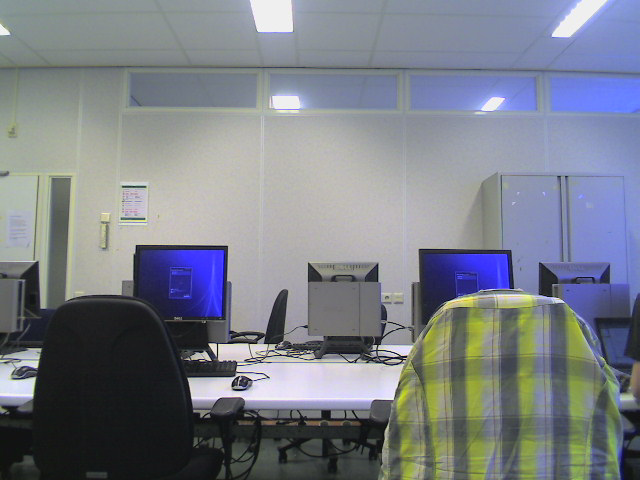
\includegraphics[width=0.4\textwidth]{leftown}
  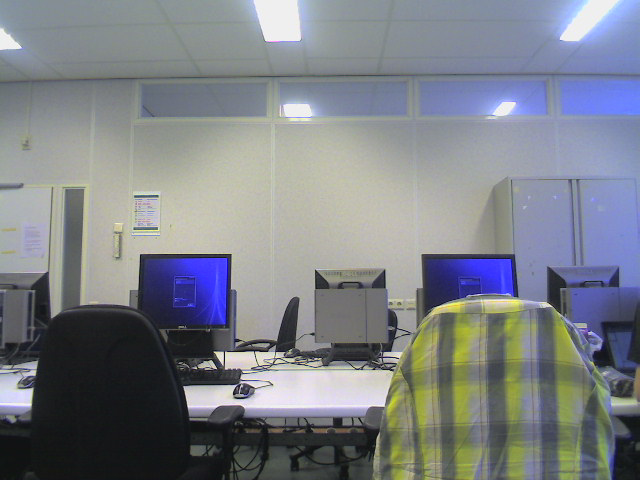
\includegraphics[width=0.4\textwidth]{rightown}
  \caption{Unrectified images}
  \label{unrectified}

  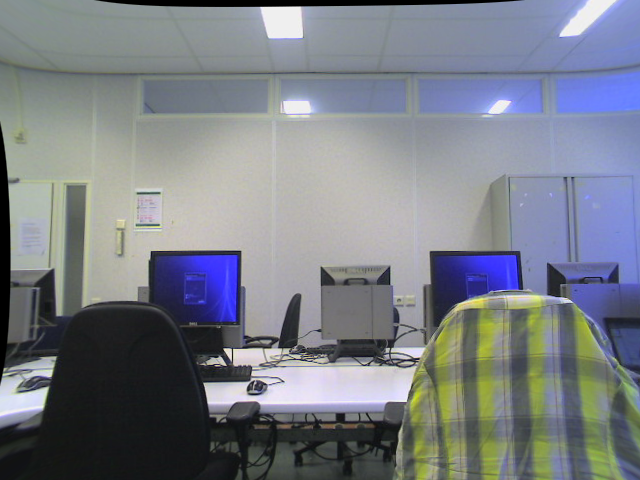
\includegraphics[width=0.4\textwidth]{leftownr}
  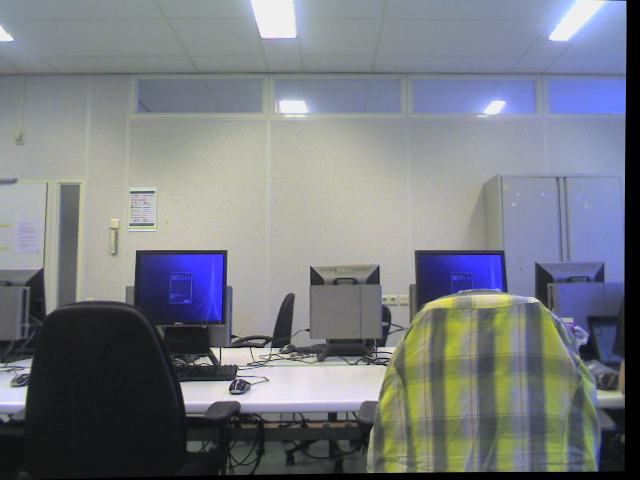
\includegraphics[width=0.4\textwidth]{rightownr}
  \caption{Rectified images}
  \label{rectified}
\end{figure} \newpage

\subsection{Rectification}
The algorithm used for rectification in OpenCV is exactly as we have
explained in the theory section (\ref{recttheory}).

\subsection{Dense Stereo Algorithms}
During our project we first started with using the standard algorithms that are
already implemented in OpenCV. As described in the theory
part of the paper (see \ref{theory}) we used three algorithms, \emph{Graph
Cut}, \emph{Block Matching} and \emph{Semi Global Block Matching}.
To test these algorithms we used the Tsukuba dataset from Middlebury
\cite{middlebury}.  This set with rectified images and their corresponding depth
maps is the standard for testing and comparing different methods of
stereo correspondence.

\subsubsection{Graph Cut}
The graph cut algorithm is one of the most popular algorithms in the
generation of disparity depth maps. We used the standard
implementation in OpenCV which is an adaptation of the Kolmogorov
paper \cite{kolmogorov2003}. Our first results almost reach the
quality of the ground truth depth map provided by the Middlebury
homepage\cite{middlebury}. See Figure \ref{gc_comp}.  Section
\ref{gc_theory} talks about the theory behind graph cut.

\begin{figure} [h!tb]
  \centering
  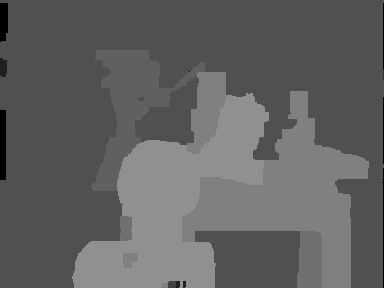
\includegraphics[width=0.4\textwidth]{gc_tsukuba_own}
  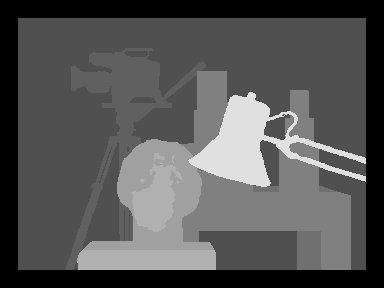
\includegraphics[width=0.4\textwidth]{disp_tsukuba_orig}
  \caption{left: Our GC depthmap, right: Middlebury Ground Truth. Gray values
  convey depth, lighter gray is closer to the camera. Black values are
  ``invalid'', meaning that using the algorithm no valid depthvalue could be
  calculated}
  \label{gc_comp}
\end{figure}

\begin{figure} [h!tb]
  \centering
  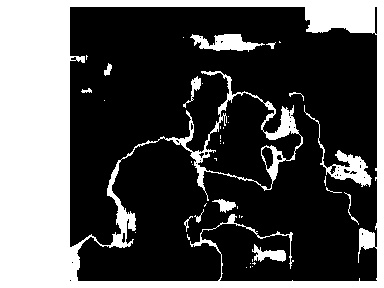
\includegraphics[width=0.4\textwidth]{bm_tsukuba_own}
  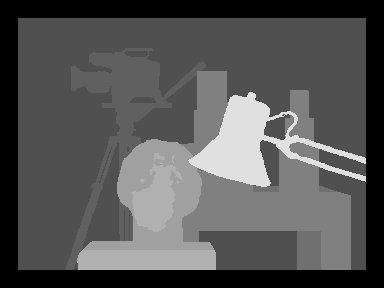
\includegraphics[width=0.4\textwidth]{disp_tsukuba_orig}
  \caption{left: Our BM depthmap, right: Middlebury Ground Truth}
  \label{bm_comp}
\end{figure}

\subsubsection{Block Matching} 
The Block Matching algorithm is much faster than the Graph Cut
Algorithm, but the quality of the results is not as good.  The quality
of the algorithm depends greatly on the configuration of the
parameters and the use of pre- and postfilters. See Figure
\ref{bm_comp} for comparison with the ground truth from Middlebury. We
couldn't find any good block matching example to compare with but with
the ground truth image you will get the idea of how it has to divide
the image into different depths.

\subsubsection{Semi Global Block Matching}
The Semi Global Block Matching algorithm is quite new in the OpenCV
library. It was implemented in version 2.1 which is the current
version at the time this article is written. It is more precise and
almost as fast as the standard block matching algorithm but the python
binding is not yet completed and integrated into OpenCV. Because of
this we wrote this part in C++. Just as the standard Block Matching
the algorithm still needs to be tuned right to return the optimal
depthmap. See Figure \ref{sgbm_comp} for comparison with the ground
truth. The tuning of the algorithm is one of the most important
steps to get good results. The tuneable parameters are: 
\begin{itemize}
\item min and max disparity
\item SAD size
\item PreFilterCap
\item disp12MaxDiff
\item uniqueness
\item speckleWindowSize and speckleRange
\item Original
\end{itemize}
\noindent\textbf{min and max disparity} are the minimum and maximum disparity
values that can be found. Between these the best one is chosen for the
disparity image. In our implementation we set the minimum disparity to
0 and the maximum disparity we chose the image width/8, because it
returned the best results\\
\textbf{SAD size} is the size of the blocks which is considered for the
Energy calculation of the algorithm. The manual suggests values
between 5 and 21 pixels. The value has to be an uneven value. We chose
a size of 9 to keep the calculation as fast as possible without too much loss of
quality.\\
\textbf{PreFilterCap} is the value for the Tomasi cost function to cap
the values at [-PreFilterCap, PreFilterCap] intervals. In the OpenCV
implementation the values given can vary between 0 and 63. We chose
for 63 because then you had the minimum noise inside the image.\\
\textbf{disp12MaxDiff} is the maximum value in the left-right
disparity check. We set it to 2 to get results that where
acceptable. More didn't make a difference and less gave much noise.\\
\textbf{uniqueness} is the switch to enable the uniqueness check. We
switched it on.\\
\textbf{speckleWindowSize} defines the maximum region which is
considered as speckle / peak. In our configuration we set the value to
100. A value less gave too much noise and a higher value didn't really
change that much. OpenCV suggests a value between 50-200.\\
\textbf{speckleRange} defines the disparity difference that is
considered as speckle. This has to be a value devidable by 16 and the
OpenCV manual suggests 16 or 32. A value of 32 gave good results.\\
\textbf{Original} at last defines if you want to use 5 or 8 paths for
the cost aggregation. We have chosen the suggested 8 paths configuration.

\begin{figure} [h!tb]
  \centering
  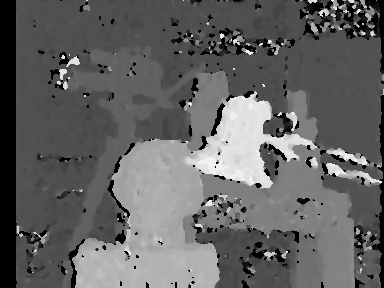
\includegraphics[width=0.4\textwidth]{sgbm_tsukuba_own}
  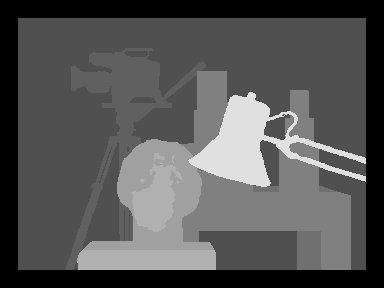
\includegraphics[width=0.4\textwidth]{disp_tsukuba_orig}
  \caption{left: Our SGBM depthmap, right: Middlebury Ground Truth}
  \label{sgbm_comp}
\end{figure}

\section{Practical problems}

\subsection{Webcams} 
We had to make the two webcams work on Linux. We had to compile our own drivers
in order to receive a live feed from both cameras at the same time.
Furthermore, because the webcams could not be moved relatively to each other
after calibration, we created a rig in which both cameras were fixed.

\subsection{OpenCV} 
We were completely unfamiliar with the library OpenCV, which we have used for
all of our calculations. We were quite accustomed to MATLAB, so it took us a
while to switch to programming linear algebra in OpenCV. First off, it took
us a while to get it working on various systems. The library is written in C,
but because we used Python bindings, it was quite hard to debug errors thrown
by the library functions.

Furthermore, in order to be able to use the SGBM functionality implemented in
the latest release of OpenCV, we had to compile our own build of the library. As
of yet, there are no binary packages available for this release. See section \ref{opencv}
for a more in depth description of OpenCV.

Besides of the OpenCV documentation, which documents each function with some comments on usage, the Learning OpenCV book \cite{LearningOpenCV} turned out to be a very useful source of information to get a good global idea of the possibilities of OpenCV in stereo vision.


\section{Applications}

\subsection{3D representation}
When taking a picture with a camera, the third dimension of depth is lost. With
a disparity depth map it is possible to reconstruct this third dimension. We
have created an OpenGL viewer that can convert a disparity depth map into a
simple 3D representation of the original image. Figure \ref{3drep}
shows screenshots of the 3D reconstruction of the Tsukuba dataset.

\begin{figure}[h!bt]
\centering
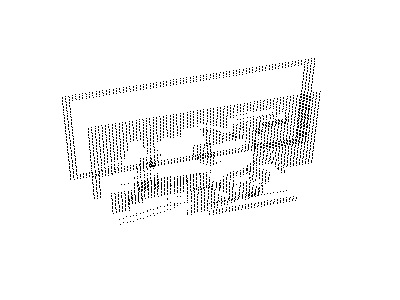
\includegraphics[width=0.4\textwidth]{3drep1}
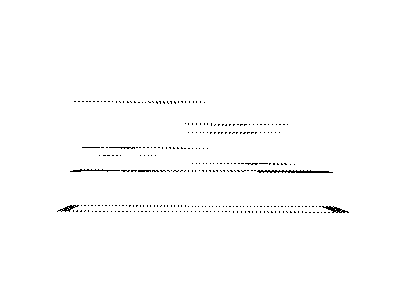
\includegraphics[width=0.4\textwidth]{3drep2}
\caption{A 3D representation of the Tsukuba dataset reconstructed from a
disparity depth map}
\label{3drep}
\end{figure}

\subsection{Remove background}
If we know the distance between the camera and an object for each pixel, we can
only show the pixels that are near enough according to some threshold distance.
Using this technique we got black images with only the front objects 'cut out'
of the original image. One could also replace the black background pixels with
an alternative image to place front objects in alternative locations. We got a
live background-removal program running which places people standing in front of
the camera at a beach or at the Efteling. Besides some noise and occlusion
problems, the images seems pretty good. See Figure \ref{remove-bg} for the
result.

\begin{figure}[h!bt]
\centering
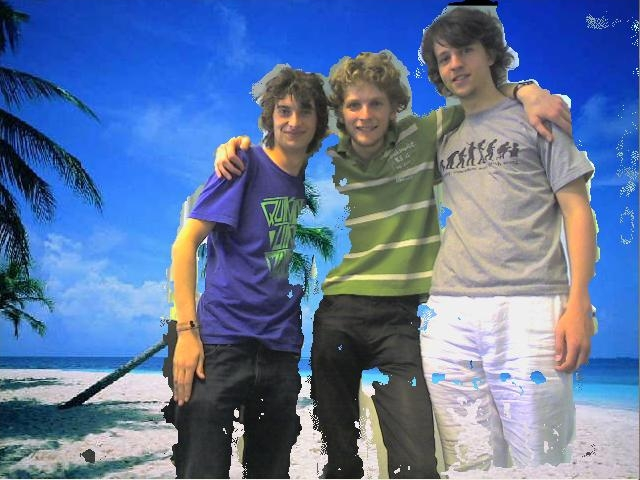
\includegraphics[width=0.6\textwidth]{remove-bg1}
\caption{Sander, Moos and Martijn on the beach in P1.24, Roeterseiland}
\label{remove-bg}
\end{figure}

\section{Further research}

\begin{description}
  \item[Applying RANSAC] We could eliminate noise when generating the disparity
  depth maps using RANSAC to reduce speckles.
  \item[Implementing BP] The newer algorithms that generate better and faster
  results all depend on Belief Propagation. It would be very nice to add this to
  our options.
  \item[Adjusting relative camera position] We would like to see what the effect
  of the relative position of the two cameras to each other is on the results.
  \item[Cube calibration] The OpenCV manual states that it is possible to
  calibrate the cameras with just one view of a 3D cube which is guaranteed to
  be straight in all directions. This would reduce the calibration steps to just
  one.
  \item[Automatic calibration] Using SIFT it is possible to calibrate without
  the use of artificial objects and interaction with the user. This would
  autonomize the program even more.
\end{description}

\newpage

\section{Planning}
This was our original planning from which we did not have to deviate greatly.

\begin{itemize}
  \item Week 1
    \begin{itemize}
      \item Reading literature
      \item Getting webcams to work
      \item Choosing dense algorithm
    \end{itemize}
  \item Week 2
    \begin{itemize}
      \item Implementing
        \begin{itemize}
          \item Dense disparity map algorithm working
          \item Camera calibration using epipolar geometry
          \item Rectification of images
        \end{itemize}
      \item Halfway report
    \end{itemize}
    
  \item Week 3
    \begin{itemize}
    \item Fine tuning camera calibration
    \item Cropping of rectified images
    \item Fine tuning parameters of dense stereo
    \item Completely understand the algorithms
    \item Depth map normalize
    \end{itemize}

  \item Week 4
    \begin{itemize}
      \item Optimizing and testing
      \item If there's enough time left
        \begin{itemize}
          \item Generate 3D image of environment
          \item Remove background using dense disparity map
        \end{itemize}
    \end{itemize}
\end{itemize}

\section{Tasks}
  \begin{itemize}
    \item Martijn and Moos
    \begin{itemize}
      \item Camera calibration
      \item Epipolar geometry
    \end{itemize}
    \item Sander and Sebastian
    \begin{itemize}
      \item Finding corresponding points
      \item Generating depth map
    \end{itemize}
  \end{itemize}

\section{NOTES MARTIJN (DELETE LATER)}

 - Calibratie beschrijft nog steeds niet echt hoe de stereo matrices (F en E)
   worden berekend, dat wil Rein eigenlijk wel. Maar daar wordt het stuk wel
   weer langer van. \\
 - De demo programma's worden nu helemaal niet beschreven. Voorstel: sectie
   'Applications' toevoegen en kort progjes beschrijven, + screenshot \\
 - Er mist nog Conclusie. \\
 - Er mist nog Reflectie. \\


\bibliographystyle{plain} \bibliography{verslag}
\end{document}
